\documentclass[11pt,a4paper]{article}

\usepackage[T1]{fontenc}
\usepackage[utf8]{inputenc}
\usepackage{lmodern}
\usepackage[margin=2.3cm]{geometry}
\usepackage{amsmath,amssymb}
\usepackage{graphicx}
\usepackage{booktabs}
\usepackage{multirow}
\usepackage{float}
\usepackage{caption}
\usepackage{xcolor}
\usepackage[hidelinks]{hyperref}

\graphicspath{{results/}}
\setlength{\parskip}{0.5em}
\setlength{\parindent}{0pt}

\newcommand{\fillme}[1]{\textcolor{red}{#1}}

% ---------------------------------------------------------------
% TIMINGS: fill these in from the FINAL run of q1.py
% ---------------------------------------------------------------
\newcommand{\timeA}{4.38}          % (a) k-means on D
\newcommand{\timeMfive}{1.73}      % (d) m = 5
\newcommand{\timeMten}{2.20}       % (d) m = 10
\newcommand{\timeMfifteen}{3.13}   % (d) m = 15
\newcommand{\timeMtwenty}{2.76}    % (d) m = 20
\newcommand{\timeMtwentyfive}{2.87}% (d) m = 25

\begin{document}

% ================= FRONT PAGE =================
\begin{titlepage}
    \centering
    \vspace*{6cm}
    {\LARGE\bfseries ASSIGNMENT 1\par}
    \vspace{0.8cm}
    {\large\bfseries\itshape (Data Science)\par}
    \vfill
    {\large\bfseries ADITRI JAIN (2024027)\par}
    \vspace{0.4cm}
    {\large\bfseries KANUPRIYA GUPTA (2023269)\par}
    \vspace{2cm}
\end{titlepage}

% ================= DATA =================
\section*{Data}

We loaded the 10\% KDD Cup 1999 data using \texttt{fetch\_kddcup99(subset=None, as\_frame=True)}.
To build $D$, we one-hot encoded \texttt{protocol\_type}, \texttt{service} and \texttt{flag}
and converted the other 38 features to float. We then dropped the two columns that have the
same value on every row (\texttt{num\_outbound\_cmds} and \texttt{is\_host\_login}) and
rescaled each column to $[0,1]$.

\begin{center}
$n = 494{,}021$ rows, \qquad $d = 116$ columns.
\end{center}

The code is in \texttt{prep.py} (data) and \texttt{q1.py} (all parts of Question 1).

% ================= QUESTION 1 =================
\section*{Question 1: JL for $k$-means clustering}

All clusterings use \texttt{KMeans(n\_clusters=15, n\_init=5, random\_state=0)}. The matrix $A$
is drawn with NumPy as \texttt{rng.normal(0, 1/np.sqrt(m), size=(m, d))}, using the seed
\texttt{np.random.default\_rng(1)} for parts (b)--(d) and \texttt{np.random.default\_rng(2)}
for part (e). Running \texttt{q1.py} again gives the same numbers (except the times).

% ---------------- (a) ----------------
\subsection*{(a)}

\begin{table}[H]
\centering
\begin{tabular}{lr}
\toprule
cost$(D,B)$ & 53{,}540.69 \\
Wall-clock time & \timeA\ s \\
\bottomrule
\end{tabular}
\caption{$k$-means on $D$.}
\end{table}

% ---------------- (b) ----------------
\subsection*{(b)}

\begin{table}[H]
\centering
\small
\begin{tabular}{clrrrrr}
\toprule
$m$ & & Run 1 & Run 2 & Run 3 & Run 4 & Run 5 \\
\midrule
\multirow{2}{*}{5}  & cost$(D,\hat B)$ & 68{,}627.41 & 62{,}564.09 & 59{,}738.25 & 56{,}108.62 & 72{,}805.03 \\
                    & ratio            & 1.2818 & 1.1685 & 1.1158 & 1.0480 & 1.3598 \\
\midrule
\multirow{2}{*}{10} & cost$(D,\hat B)$ & 53{,}438.76 & 60{,}751.89 & 58{,}228.92 & 59{,}565.60 & 52{,}916.48 \\
                    & ratio            & 0.9981 & 1.1347 & 1.0876 & 1.1125 & 0.9883 \\
\midrule
\multirow{2}{*}{15} & cost$(D,\hat B)$ & 55{,}120.00 & 52{,}859.53 & 55{,}815.34 & 55{,}024.33 & 53{,}824.66 \\
                    & ratio            & 1.0295 & 0.9873 & 1.0425 & 1.0277 & 1.0053 \\
\midrule
\multirow{2}{*}{20} & cost$(D,\hat B)$ & 56{,}651.59 & 59{,}784.80 & 53{,}279.89 & 52{,}062.00 & 54{,}225.08 \\
                    & ratio            & 1.0581 & 1.1166 & 0.9951 & 0.9724 & 1.0128 \\
\midrule
\multirow{2}{*}{25} & cost$(D,\hat B)$ & 55{,}094.72 & 55{,}524.17 & 52{,}932.59 & 55{,}258.92 & 54{,}503.53 \\
                    & ratio            & 1.0290 & 1.0370 & 0.9886 & 1.0321 & 1.0180 \\
\bottomrule
\end{tabular}
\caption{cost$(D,\hat B)$ and cost$(D,\hat B)/\text{cost}(D,B)$ for each run.}
\end{table}

\begin{table}[H]
\centering
\begin{tabular}{c ccc ccc}
\toprule
 & \multicolumn{3}{c}{cost$(D,\hat B)/\text{cost}(D,B)$} & \multicolumn{3}{c}{cost$(D,B^+)/\text{cost}(D,B)$} \\
\cmidrule(lr){2-4}\cmidrule(lr){5-7}
$m$ & Mean & Min & Max & Mean & Min & Max \\
\midrule
5  & 1.1948 & 1.0480 & 1.3598 & 80.36 & 79.67 & 81.27 \\
10 & 1.0642 & 0.9883 & 1.1347 & 76.10 & 74.64 & 77.71 \\
15 & 1.0185 & 0.9873 & 1.0425 & 70.51 & 66.20 & 72.34 \\
20 & 1.0310 & 0.9724 & 1.1166 & 71.46 & 69.20 & 74.01 \\
25 & 1.0210 & 0.9886 & 1.0370 & 63.85 & 59.74 & 66.08 \\
\bottomrule
\end{tabular}
\caption{Mean, smallest and largest ratio over the 5 runs, for $\hat B$ (part b) and $B^+$ (part c).}
\label{tab:summary}
\end{table}

\textbf{How the ratio changes with $m$.} As $m$ increases, the ratio gets closer to 1.
At $m=5$ the clustering is clearly worse than $k$-means on $D$ (mean 1.19, worst run 1.36).
At $m=10$ the mean drops to 1.06, and from $m=15$ onwards it stays around 1.02--1.03 with a
smaller gap between the best and worst runs. This is what we expected. With more dimensions,
the random projection keeps the distances between points more accurately, and since the
$k$-means cost only depends on these distances, the clusters found on $E$ are almost as good
as the ones found on $D$. The mean at $m=20$ is slightly higher than at $m=15$ because of one
bad run (1.1166). With only 5 runs per $m$, this is just random variation.

\textbf{Ratios below 1.} Six runs have a ratio below 1, the lowest being 0.9724 at $m=20$.
This can happen because $k$-means only finds a local optimum, so $B$ is not the best possible
set of centres, and the clustering found on $E$ can sometimes end up slightly better. Also,
when we compute cost$(D,\hat B)$, every point is reassigned to its nearest centre in $\hat B$,
which can only lower the cost.

% ---------------- (c) ----------------
\subsection*{(c)}

The ratio cost$(D,B^+)/\text{cost}(D,B)$ is shown next to the ratio for $\hat B$ in
Table~\ref{tab:summary}. It is between 59.7 and 81.3 in every run, while the ratio for
$\hat B$ is close to 1.

The reason is that the centre $k$-means finds on $E$ is (almost exactly) $A\hat b_j$, so
$A^+a \approx A^+A\,\hat b_j$. The matrix $A^+A$ projects onto an $m$-dimensional subspace,
so $B^+$ only keeps the part of each centre that lies in that subspace and loses the rest.
The centres shrink towards the origin and end up far from the data, which makes the cost very
large. It gets a little better as $m$ grows (about 80 at $m=5$ to 64 at $m=25$) because more
of each centre is kept.

We would use $\hat B$, since its cost is almost the same as that of $k$-means on $D$.

% ---------------- (d) ----------------
\subsection*{(d)}

\begin{table}[H]
\centering
\begin{tabular}{lccccc}
\toprule
$m$ & 5 & 10 & 15 & 20 & 25 \\
\midrule
Mean time (s) & \timeMfive & \timeMten & \timeMfifteen & \timeMtwenty & \timeMtwentyfive \\
\bottomrule
\end{tabular}
\caption{Time to compute $E$ and run $k$-means on $E$, averaged over the 5 runs.
$k$-means on $D$ took \timeA\ s.}
\label{tab:time}
\end{table}

\begin{figure}[H]
\centering
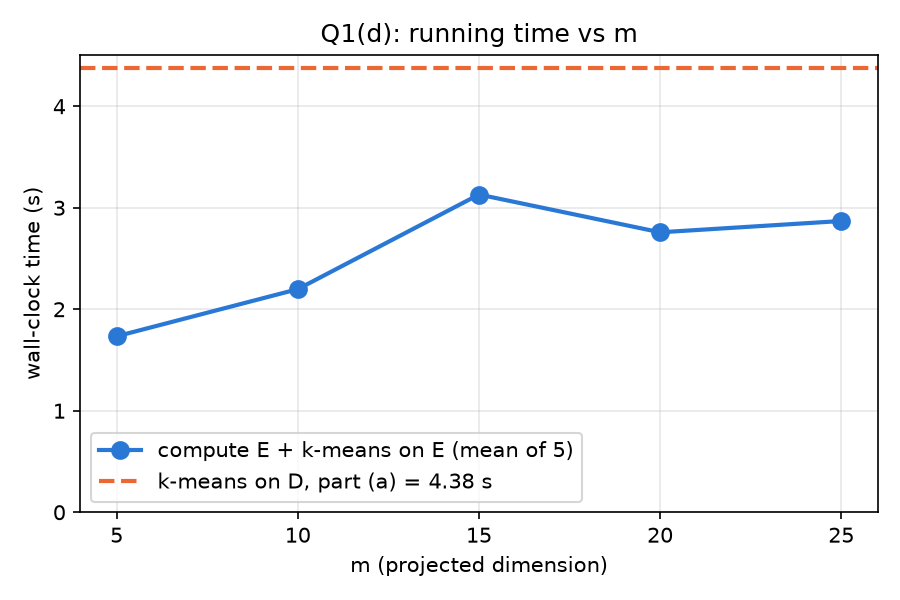
\includegraphics[width=0.7\textwidth]{q1d_time.png}
\caption{Mean time against $m$. The dashed line is the time of $k$-means on $D$ from (a).}
\end{figure}

For every $m$, computing $E$ and running $k$-means on it was faster than $k$-means on $D$
(\timeA\ s). It took 1.73 s at $m=5$, which is about 2.5 times faster, and between 2.2 and
3.1 s for the larger values of $m$. The time mostly goes up with $m$, since each distance
computation uses $m$ coordinates. The value at $m=15$ is a bit higher than at $m=20$ and $25$
because of one slower run (4.29 s). Computing $E$ itself takes very little time (about 0.1 s).

The speedup is much smaller than $d/m$ (for example $116/5 \approx 23$). Part of the work in
$k$-means does not depend on the dimension, and at small $m$ the clusters overlap more, so
$k$-means sometimes needs more iterations to converge.

% ---------------- (e) ----------------
\subsection*{(e)}

We picked $10^4$ random pairs once, skipping any pair with $D_i = D_l$, and used the same pairs
for every $m$.

\begin{figure}[H]
\centering
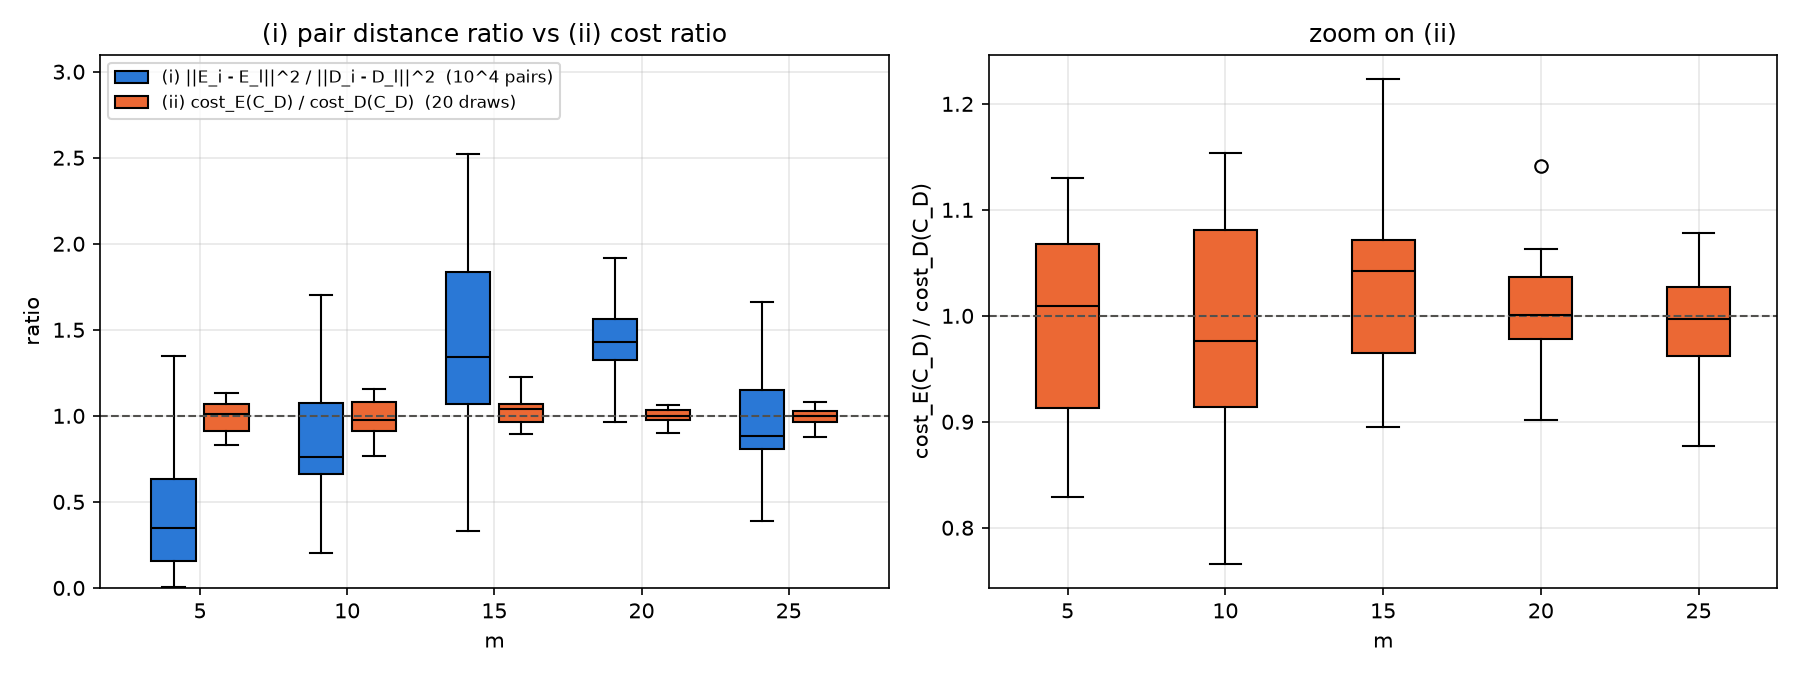
\includegraphics[width=\textwidth]{q1e_boxplots.png}
\caption{Left: ratio (i) (blue) and ratio (ii) (orange) against $m$. Right: ratio (ii) on
its own scale, since its boxes are too small to see on the left. Outliers of (i) are not drawn.}
\end{figure}

\begin{table}[H]
\centering
\begin{tabular}{clrrrrr}
\toprule
$m$ & Ratio & Mean & Median & Std & Min & Max \\
\midrule
\multirow{2}{*}{5}  & (i) pairs & 0.4403 & 0.3476 & 0.4076 & 0.0071 & 2.7302 \\
                    & (ii) cost & 0.9939 & 1.0093 & 0.0961 & 0.8293 & 1.1305 \\
\midrule
\multirow{2}{*}{10} & (i) pairs & 0.9030 & 0.7602 & 0.3589 & 0.2035 & 2.7880 \\
                    & (ii) cost & 0.9789 & 0.9765 & 0.1101 & 0.7661 & 1.1538 \\
\midrule
\multirow{2}{*}{15} & (i) pairs & 1.3372 & 1.3401 & 0.4464 & 0.3318 & 2.5196 \\
                    & (ii) cost & 1.0313 & 1.0425 & 0.0745 & 0.8953 & 1.2237 \\
\midrule
\multirow{2}{*}{20} & (i) pairs & 1.3789 & 1.4266 & 0.2743 & 0.3589 & 1.9541 \\
                    & (ii) cost & 1.0083 & 1.0006 & 0.0512 & 0.9016 & 1.1416 \\
\midrule
\multirow{2}{*}{25} & (i) pairs & 0.9490 & 0.8855 & 0.2179 & 0.3860 & 2.1907 \\
                    & (ii) cost & 0.9908 & 0.9971 & 0.0501 & 0.8776 & 1.0779 \\
\bottomrule
\end{tabular}
\caption{Summary of the ratios: (i) over $10^4$ pairs with one draw of $A$, (ii) over 20 draws of $A$.}
\end{table}

\textbf{Which has the smaller spread.} The cost ratio (ii) has a much smaller spread than the
pair ratio (i) for every $m$. Its standard deviation is between 0.05 and 0.11 and it stays close
to 1. The pair ratio has a standard deviation between 0.22 and 0.45, and single values go from
almost 0 up to about 2.8. One random $A$ can stretch or shrink the distance of a single pair a
lot, but the clustering cost adds up the distances of all 494,021 points to their cluster means,
so the errors in different directions cancel out.

\textbf{How each changes with $m$.} The spread of (ii) goes down as $m$ grows: the standard
deviation is about 0.10 for $m=5$ and $10$ and about 0.05 for $m=20$ and $25$. The spread of (i)
also goes down overall (the range goes from $[0.007,\ 2.73]$ at $m=5$ to $[0.39,\ 2.19]$ at
$m=25$), but not smoothly, and its median is far from 1 for some values of $m$ (0.35 at $m=5$,
1.43 at $m=20$). This is because, for each $m$, all $10^4$ pairs use the same single $A$. Most of
the pairs are of a few types (such as neptune--smurf and normal--smurf), so their differences
point in similar directions, and one $A$ moves most of them up or down together.

% ================= QUESTION 2 =================
% This file is generated by make_q2_tex.py from the results of Q2_JL_linear_regression.ipynb.
\clearpage
\section*{Question 2: JL for linear regression}

We use the same $D$ as in Question 1 (see Data), with $n = 494{,}021$ rows and $d = 116$ columns. The label is
$y_i = 1$ if connection $i$ is an attack (its label is not \texttt{normal.}) and $y_i = 0$ otherwise,
which gives 396{,}743 attacks and 97{,}278 normal connections (80.3\% attacks).
The notebook for this question builds $D$ with the same three steps, and we checked that the result is
identical to the output of \texttt{prep.py}.

Every least-squares problem is solved with \texttt{numpy.linalg.lstsq(M, z, rcond=None)}. The random
numbers come from \texttt{np.random.SeedSequence(558).spawn(6)}: one generator each for (b), (d),
the subset in (e), the CountSketches in (e), the Gaussian sketches in (e), and the extra check on the full
$D$ in (e). Running the notebook again gives the same losses and ratios (except the times). The code is in
\texttt{q2/Q2\_JL\_linear\_regression.ipynb}. All times are on an Apple M4.

\textbf{Rank of $D$.} $\operatorname{rank}(D) = 113$, not 116, because of three exact linear relations
between the one-hot columns. The \texttt{protocol\_type}, \texttt{service} and \texttt{flag} columns each
add up to the all-ones vector (two independent relations), and \texttt{protocol\_type\_icmp} equals the sum
of the six ICMP-only service columns (\texttt{eco\_i}, \texttt{ecr\_i}, \texttt{red\_i}, \texttt{tim\_i},
\texttt{urh\_i}, \texttt{urp\_i}). The notebook checks all three. We write $r = \operatorname{rank}(D) = 113$
and $L^* = \text{Loss}(D,y,b)$. Since the all-ones vector is in the column space of $D$, the model already
has an intercept.

\textbf{Why sketch-and-solve works.} Instead of solving $\min_a \|Da-y\|_2^2$, which has $n$ equations,
we solve $\min_a \|SDa-Sy\|_2^2$, which has only $m$. Every vector $Da-y$ lies in
$W = \operatorname{span}(\text{columns of } D,\ y)$, a fixed subspace of dimension at most $r+1$.
Suppose that for every $w \in W$,
$(1-\varepsilon)\|w\|^2 \le \|Sw\|^2 \le (1+\varepsilon)\|w\|^2$. Then
\[
\text{Loss}(D,y,\tilde a)
\le \frac{\|S(D\tilde a-y)\|^2}{1-\varepsilon}
\le \frac{\|S(Db-y)\|^2}{1-\varepsilon}
\le \frac{1+\varepsilon}{1-\varepsilon}\,\text{Loss}(D,y,b),
\]
where the middle step holds because $\tilde a$ minimises the sketched loss. So we need the JL property for
a whole subspace, not for $n$ fixed points. This is impossible when $m < r$, since some nonzero $Dz$ is then
mapped to $0$. A Gaussian $S$ works with $m = O((r+\log(1/\delta))/\varepsilon^2)$ and a CountSketch with
$m = O(r^2/(\delta\varepsilon^2))$ (Clarkson and Woodruff, 2013), but $SD$ for a CountSketch costs only one
pass over $D$.

% ---------------- (a) ----------------
\subsection*{(a)}

\begin{enumerate}
    \item Solve $b = \arg\min_a \|Da-y\|_2^2$ with \texttt{lstsq} on the full $D$. Because
    $\operatorname{rank}(D) = 113 < 116$, the minimiser is not unique. \texttt{lstsq} returns the one with
    the smallest norm, and the minimum loss is the same for all of them.
    \item Time the call with \texttt{time.perf\_counter}, 5 times, and take the mean.
\end{enumerate}

\begin{table}[H]
\centering
\begin{tabular}{lr}
\toprule
Loss$(D,y,b) = \|Db-y\|_2^2$ & 2{,}949.79 \\
Loss of the best constant, $\|y-\bar y\|_2^2$ & 78{,}122.9 \\
$\|b\|_2$ (minimum-norm solution) & 135.3 \\
Wall-clock time (mean of 5 runs) & 1.61~s \\
\bottomrule
\end{tabular}
\caption{Least squares on the full $D$. The 5 times were 1.71, 1.53, 1.53, 1.67 and 1.59~s.}
\end{table}

Loss$(D,y,b) = 2{,}949.79$ and computing $b$ takes 1.61~s. For scale, predicting the constant $\bar y$
gives a loss of 78{,}122.9, so the linear fit explains $1 - L^*/\|y-\bar y\|^2 = 0.962$ of the variance of $y$.

% ---------------- (b) ----------------
\subsection*{(b)}

\begin{enumerate}
    \item \textbf{Draw $S$.} For each row $i$, draw a bucket $h(i) \in \{1,\dots,m\}$ and a sign
    $\sigma(i) \in \{-1,+1\}$, uniformly and independently. $S$ is stored as these two arrays of length $n$,
    never as an $m \times n$ matrix.
    \item \textbf{Form $SD$ and $Sy$ in one pass.} Row $i$ of $D$, times $\sigma(i)$, is added to row $h(i)$ of
    $SD$ with \texttt{np.add.at(SD, h, sigma[:, None] * D)}, and the same for $y$. A test in the notebook checks
    this against an explicit dense $S$.
    \item \textbf{Solve} $\tilde a = \arg\min_a \|SDa-Sy\|_2^2$ with \texttt{lstsq}.
    \item \textbf{Record} Loss$(D,y,\tilde a)$, its ratio to $L^*$ and the sketched loss $\|SD\tilde a-Sy\|_2^2$.
    To explain the results we also record $\operatorname{rank}(SD)$, the smallest nonzero singular value
    $\sigma_{\min}(SD)$ and $\|\tilde a\|_2$.
    \item Repeat 5 times for each $m$, with a new $S$ each time (35 runs).
\end{enumerate}

\begin{table}[H]
\centering
\small
\begin{tabular}{clrrrrr}
\toprule
$m$ & & Run 1 & Run 2 & Run 3 & Run 4 & Run 5 \\
\midrule
\multirow{3}{*}{50} & Loss$(D,y,\tilde a)$ & 11{,}498.80 & 7{,}264.36 & 11{,}411.00 & 12{,}073.95 & 12{,}097.89 \\
     & ratio & 3.8982 & 2.4627 & 3.8684 & 4.0932 & 4.1013 \\
     & sketched loss & $5.8\times10^{-24}$ & $9.3\times10^{-25}$ & $4.8\times10^{-24}$ & $1.0\times10^{-23}$ & $3.3\times10^{-24}$ \\
\midrule
\multirow{3}{*}{100} & Loss$(D,y,\tilde a)$ & 32{,}883.33 & 20{,}199.80 & 66{,}338.88 & 65{,}310.47 & 26{,}236.80 \\
     & ratio & 11.1477 & 6.8479 & 22.4894 & 22.1407 & 8.8945 \\
     & sketched loss & $1.7\times10^{-23}$ & $3.2\times10^{-24}$ & $1.3\times10^{-22}$ & $5.0\times10^{-23}$ & $2.2\times10^{-23}$ \\
\midrule
\multirow{3}{*}{200} & Loss$(D,y,\tilde a)$ & 6{,}047.56 & 7{,}982.18 & 6{,}928.03 & 7{,}613.69 & 6{,}586.72 \\
     & ratio & 2.0502 & 2.7060 & 2.3487 & 2.5811 & 2.2329 \\
     & sketched loss & 1{,}134.17 & 1{,}210.64 & 1{,}471.30 & 1{,}101.11 & 1{,}404.11 \\
\midrule
\multirow{3}{*}{500} & Loss$(D,y,\tilde a)$ & 3{,}846.66 & 3{,}852.79 & 3{,}571.10 & 3{,}795.08 & 3{,}823.36 \\
     & ratio & 1.3040 & 1.3061 & 1.2106 & 1.2866 & 1.2961 \\
     & sketched loss & 2{,}364.48 & 2{,}002.69 & 2{,}545.48 & 2{,}158.95 & 2{,}491.13 \\
\midrule
\multirow{3}{*}{1000} & Loss$(D,y,\tilde a)$ & 3{,}350.47 & 3{,}294.78 & 3{,}351.69 & 3{,}283.23 & 3{,}317.79 \\
     & ratio & 1.1358 & 1.1170 & 1.1362 & 1.1130 & 1.1248 \\
     & sketched loss & 2{,}692.79 & 2{,}744.54 & 2{,}634.58 & 2{,}466.63 & 2{,}447.48 \\
\midrule
\multirow{3}{*}{2000} & Loss$(D,y,\tilde a)$ & 3{,}106.72 & 3{,}113.09 & 3{,}169.98 & 3{,}114.72 & 3{,}094.90 \\
     & ratio & 1.0532 & 1.0554 & 1.0746 & 1.0559 & 1.0492 \\
     & sketched loss & 2{,}706.59 & 2{,}763.15 & 2{,}848.84 & 2{,}774.54 & 2{,}652.60 \\
\midrule
\multirow{3}{*}{5000} & Loss$(D,y,\tilde a)$ & 3{,}015.98 & 3{,}021.00 & 3{,}024.20 & 3{,}014.93 & 3{,}030.11 \\
     & ratio & 1.0224 & 1.0241 & 1.0252 & 1.0221 & 1.0272 \\
     & sketched loss & 2{,}922.98 & 2{,}913.55 & 2{,}859.09 & 2{,}908.99 & 2{,}973.70 \\
\bottomrule
\end{tabular}
\caption{Loss$(D,y,\tilde a)$, ratio $=$ Loss$(D,y,\tilde a)/L^*$ and sketched loss $\|SD\tilde a-Sy\|_2^2$
for each run ($L^* = 2{,}949.79$).}
\end{table}

\begin{table}[H]
\centering
\small
\setlength{\tabcolsep}{4.5pt}
\begin{tabular}{r rrrr rr rrr}
\toprule
 & \multicolumn{4}{c}{Loss$(D,y,\tilde a)/L^*$} & \multicolumn{2}{c}{sketched loss$/L^*$} & & & \\
\cmidrule(lr){2-5}\cmidrule(lr){6-7}
$m$ & Mean & Min & Max & Ref. & Mean & Ref. & $\operatorname{rank}(SD)$ & $\sigma_{\min}(SD)$ & $\|\tilde a\|_2$ \\
\midrule
50 & 3.685 & 2.463 & 4.101 & -- & $1.7\times10^{-27}$ & 0 & 50 & 5.405 & 4.7 \\
100 & 14.304 & 6.848 & 22.489 & -- & $1.5\times10^{-26}$ & 0 & 100 & 0.382 & 24.4 \\
200 & 2.384 & 2.050 & 2.706 & 2.314 & 0.429 & 0.435 & 113 & 0.070 & 177.6 \\
500 & 1.281 & 1.211 & 1.306 & 1.293 & 0.784 & 0.774 & 113 & 0.094 & 149.4 \\
1000 & 1.125 & 1.113 & 1.136 & 1.128 & 0.880 & 0.887 & 113 & 0.101 & 142.9 \\
2000 & 1.058 & 1.049 & 1.075 & 1.060 & 0.932 & 0.944 & 113 & 0.104 & 134.5 \\
5000 & 1.024 & 1.022 & 1.027 & 1.023 & 0.988 & 0.977 & 113 & 0.105 & 134.3 \\
\bottomrule
\end{tabular}
\caption{Mean, smallest and largest ratio over the 5 runs, the mean sketched loss, and the mean of the three
extra quantities. The two ``Ref.'' columns are the exact means for a dense Gaussian $S$, derived at the end
of this part. For comparison, $\sigma_{\min}(D) = 0.106$ and $\|b\|_2 = 135.3$.}
\label{tab:q2b}
\end{table}

\begin{figure}[H]
\centering
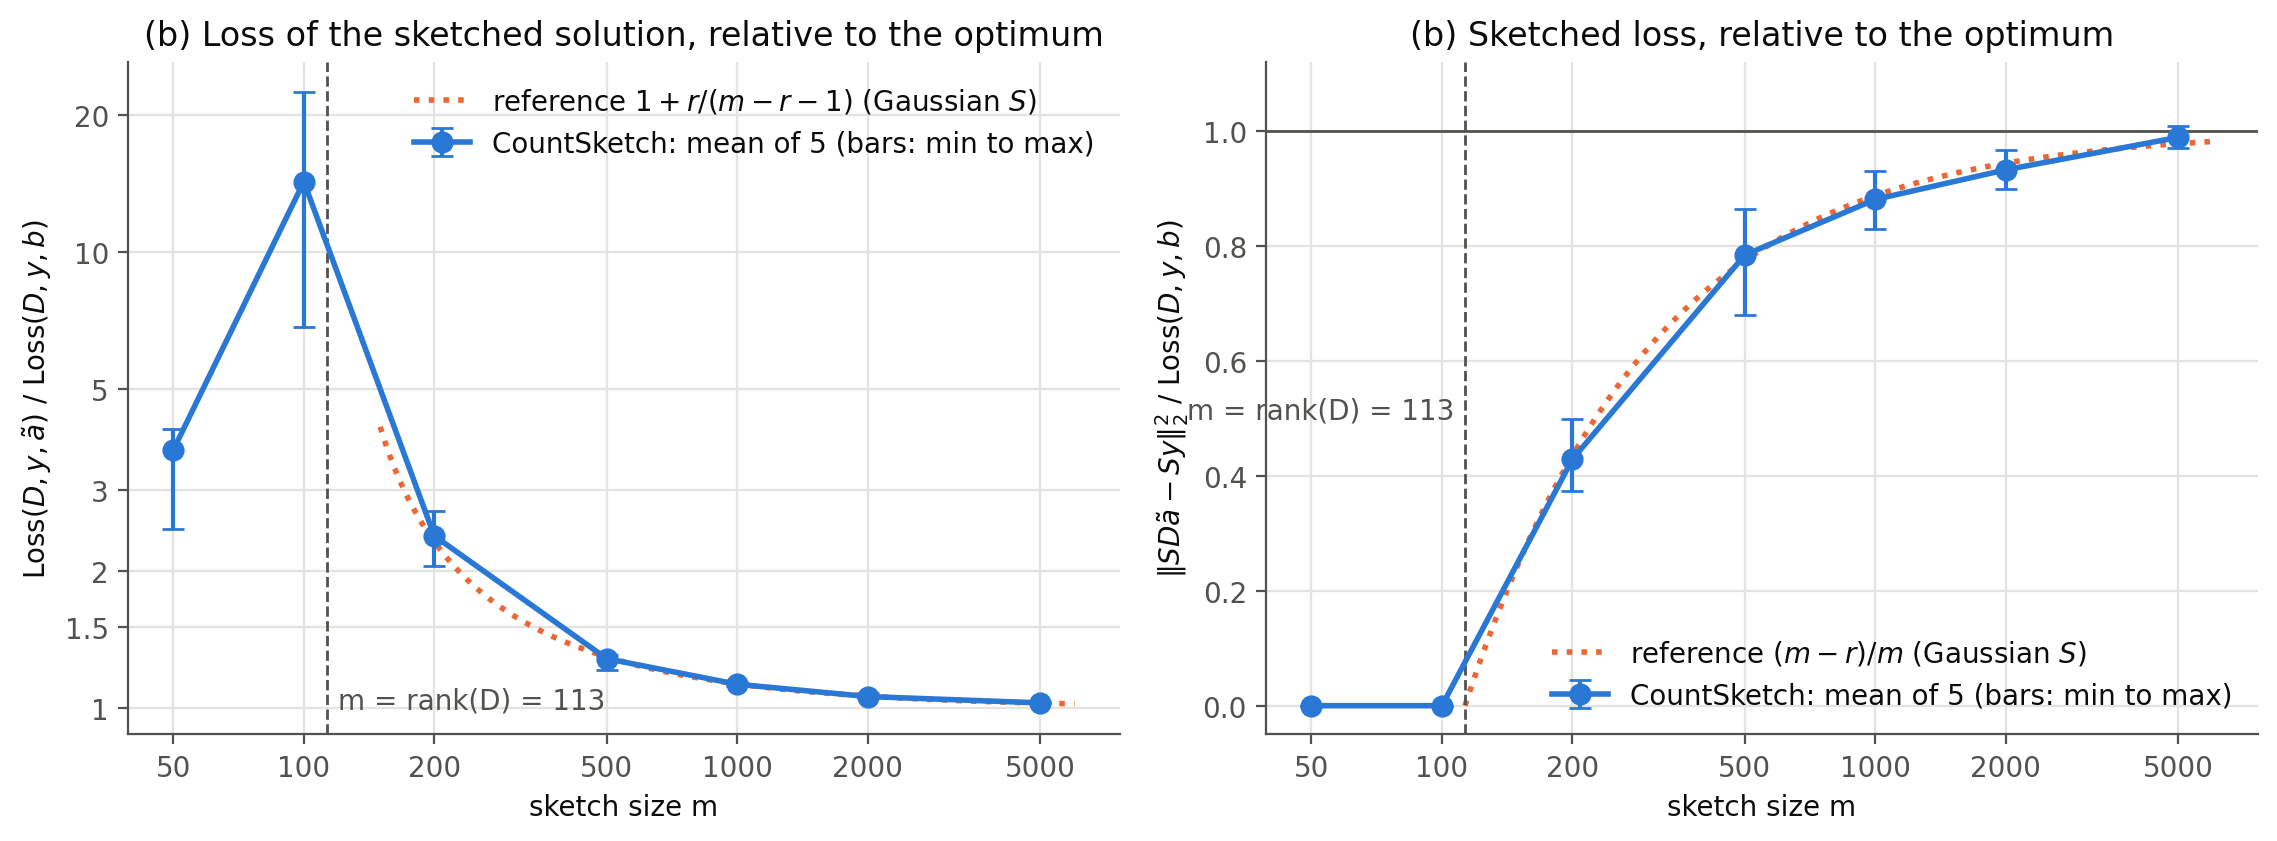
\includegraphics[width=\textwidth]{q2b_ratio_loglog.png}
\caption{Left: mean ratio Loss$(D,y,\tilde a)/L^*$ against $m$ on log--log axes; the bars go from the smallest
to the largest of the 5 runs. Right: the sketched loss divided by $L^*$. The dashed line is at
$m = \operatorname{rank}(D) = 113$.}
\end{figure}

\textbf{Below $m = \operatorname{rank}(D) = 113$ ($m = 50, 100$).}
\begin{itemize}
    \item \textbf{The sketched loss is zero.} $SD$ is $m \times 116$ with rank $m$ in every run, so the $m$
    equations $SDa = Sy$ can be solved exactly. The sketched loss is between $9.3\times10^{-25}$ and $1.3\times10^{-22}$, which is
    zero up to rounding, while the true loss is in the thousands.
    \item \textbf{The ratio is large and varies a lot}: 3.68 (2.46 to 4.10) at $m = 50$ and
    14.3 (6.8 to 22.5) at $m = 100$. $S$ maps a subspace of $\operatorname{col}(D)$ of dimension
    at least $r-m$ to $0$, so the sketched problem cannot see those directions, and \texttt{lstsq} just returns
    the minimum-norm point among a whole family of exact solutions.
    \item \textbf{It gets worse as $m$ gets close to $r$.} At $m = 100$ the sketch has to fit 100 equations
    exactly with barely more useful unknowns (113), so the equations are close to dependent:
    $\sigma_{\min}(SD)$ falls from 5.4 at $m = 50$ to 0.38 at $m = 100$. Fitting the sketched noise
    exactly then needs large coefficients ($\|\tilde a\|_2$ grows from 4.7 to 24.4), and the true
    loss blows up. This peak just below $m = \operatorname{rank}(D)$ is known as the interpolation threshold
    (or ``double descent'').
\end{itemize}

\textbf{Above $m = \operatorname{rank}(D)$ ($m = 200$, $500$, $1000$, $2000$ and $5000$).}
\begin{itemize}
    \item $\operatorname{rank}(SD) = 113 = \operatorname{rank}(D)$ in all 25 runs, so $S$ is one-to-one on
    $\operatorname{col}(D)$ and the sketched problem is overdetermined. As $m$ grows, $\sigma_{\min}(SD)$ gets
    close to $\sigma_{\min}(D) = 0.106$ (0.070 at $m = 200$, 0.105 at
    $m = 5000$), i.e.\ $S$ becomes a better subspace embedding.
    \item \textbf{The ratio falls steadily towards 1}: 2.384 $\to$ 1.281 $\to$ 1.125 $\to$ 1.058 $\to$ 1.024, and the gap between the best and worst
    run shrinks too. It follows $1 + r/(m-r-1) \approx 1 + r/m$, so the extra loss roughly halves when $m$
    doubles. On the log--log plot the curve flattens out towards 1 from above.
    \item \textbf{No ratio is below 1}, in any of the 35 runs, and none can be: $b$ minimises
    Loss$(D,y,\cdot)$ over all $a$, so Loss$(D,y,\tilde a) \ge$ Loss$(D,y,b)$ for every $\tilde a$.
    \item \textbf{The sketched loss is no longer zero and rises towards $L^*$ from below.} Divided by $L^*$
    it goes 0.43 $\to$ 0.78 $\to$ 0.88 $\to$ 0.93 $\to$ 0.99, close to $(m-r)/m$. It is always an underestimate:
    $\|SD\tilde a-Sy\|^2 \le \|S(Db-y)\|^2 \approx \|Db-y\|^2$, and the $r$ fitted coefficients absorb about a
    fraction $r/m$ of the sketched residual.
\end{itemize}

\textbf{Where the reference values come from.} Take a dense Gaussian $S$ with $N(0,1/m)$ entries and
$m > r+1$. Let $U \in \mathbb{R}^{n\times r}$ be an orthonormal basis of $\operatorname{col}(D)$, write
$Db = Uc_b$, and let $v = Db-y$, which is orthogonal to $\operatorname{col}(D)$.
\begin{enumerate}
    \item Every fitted vector is $Da = Uc$, and by Pythagoras Loss$(D,y,a) = \|v\|^2 + \|c-c_b\|^2$.
    \item $Sy = SUc_b - Sv$, so the sketched solution is $\tilde c = c_b - (SU)^+Sv$ and
    Loss$(D,y,\tilde a) - L^* = \|(SU)^+Sv\|^2$.
    \item Because $U \perp v$, the Gaussian matrices $SU$ and $Sv \sim N(0, \tfrac{\|v\|^2}{m} I_m)$ are
    independent. Using $\mathbb{E}\big[((SU)^\top SU)^{-1}\big] = \tfrac{m}{m-r-1} I_r$ (inverse Wishart),
    $\mathbb{E}\|(SU)^+Sv\|^2 = \tfrac{\|v\|^2}{m}\operatorname{tr}\mathbb{E}\big[((SU)^\top SU)^{-1}\big]
    = \|v\|^2\,\tfrac{r}{m-r-1}$. So the mean ratio is $1 + \tfrac{r}{m-r-1}$.
    \item The sketched loss is $\|(I-P)Sv\|^2$, where $P$ is the projection onto the $r$-dimensional
    $\operatorname{col}(SU)$, which is independent of $Sv$. So its mean is $\|v\|^2\,\tfrac{m-r}{m}$.
\end{enumerate}
The CountSketch results in Table~\ref{tab:q2b} are close to both reference values.

% ---------------- (c) ----------------
\subsection*{(c)}

In each run of (b) we timed three steps separately: drawing $S$ ($h$ and $\sigma$), forming $SD$ and $Sy$,
and solving the $m \times 116$ problem.

\begin{table}[H]
\centering
\begin{tabular}{rrrrrr}
\toprule
$m$ & Draw $S$ (ms) & Form $SD$, $Sy$ (ms) & Solve (ms) & Total (s) & Speed-up vs (a) \\
\midrule
50 & 4.2 & 433 & 0.4 & 0.438 & 3.7$\times$ \\
100 & 7.1 & 440 & 1.0 & 0.448 & 3.6$\times$ \\
200 & 6.7 & 478 & 4.8 & 0.490 & 3.3$\times$ \\
500 & 5.9 & 469 & 3.6 & 0.478 & 3.4$\times$ \\
1000 & 5.4 & 484 & 7.8 & 0.497 & 3.2$\times$ \\
2000 & 4.9 & 452 & 3.7 & 0.461 & 3.5$\times$ \\
5000 & 4.0 & 442 & 8.1 & 0.454 & 3.5$\times$ \\
\bottomrule
\end{tabular}
\caption{Time of sketch-and-solve, averaged over the 5 runs of (b). Computing $b$ in (a) took 1.61~s.}
\end{table}

\begin{figure}[H]
\centering
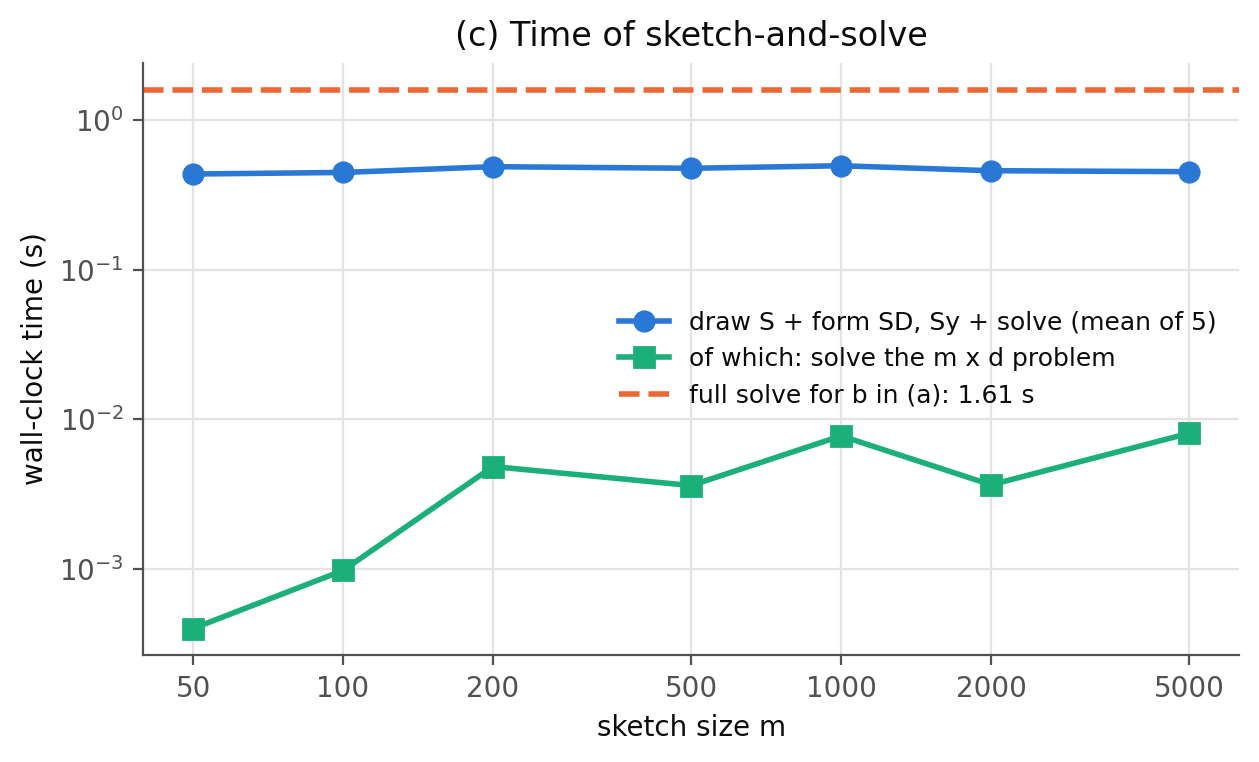
\includegraphics[width=0.7\textwidth]{q2c_times.png}
\caption{Total sketch-and-solve time (mean of 5 runs) and the solve step alone, against the time of the full
solve from (a).}
\end{figure}

Sketch-and-solve takes 0.44--0.50~s for every $m$, against 1.61~s for the full solve, so it is
about 3.2--3.7 times faster.
\begin{itemize}
    \item \textbf{Forming $SD$ and $Sy$ takes most of the time} (at least 97\%, about 0.46~s),
    and it does not depend on $m$. It is one pass over the $nd \approx 57.3$ million entries of $D$: each row is
    added once, wherever it lands.
    \item Drawing $S$ needs only $2n$ random numbers (about 5~ms). Solving the small problem costs
    $O(md^2)$. It grows with $m$ (0.4 to 8.1~ms) but stays a few percent of the total.
    \item The full solve costs $O(nd^2) \approx 6.6\times10^9$ operations, against $O(nd + md^2)$ for the
    sketch, so we expected a larger speed-up. It is only 3.2--3.7 times because $d = 116$ is small,
    the SVD inside \texttt{lstsq} is very fast, and \texttt{np.add.at} works one element at a time (about
    8 ns per entry). The gap would be larger for a bigger $d$, or for a sparse $D$, where the sketch
    costs $O(\operatorname{nnz}(D))$.
    \item Together with (b): in about a third of the time, $m = 1000$ gives a loss within 1.125 times the
    optimum and $m = 5000$ within 1.024 times.
\end{itemize}

% ---------------- (d) ----------------
\subsection*{(d)}

\begin{enumerate}
    \item Compute $v = Db-y$ once, so $\|v\|^2 = L^*$. It is fixed before any $S$ is drawn, which is exactly
    the setting of the JL lemma.
    \item For $m \in \{50, 500, 5000\}$, draw 100 independent CountSketches, form $Sv$ in one pass, and record
    $\|Sv\|_2^2/\|v\|_2^2$.
    \item Plot a histogram for each $m$ on the same $x$-axis, so the spreads can be compared directly.
\end{enumerate}

\begin{figure}[H]
\centering
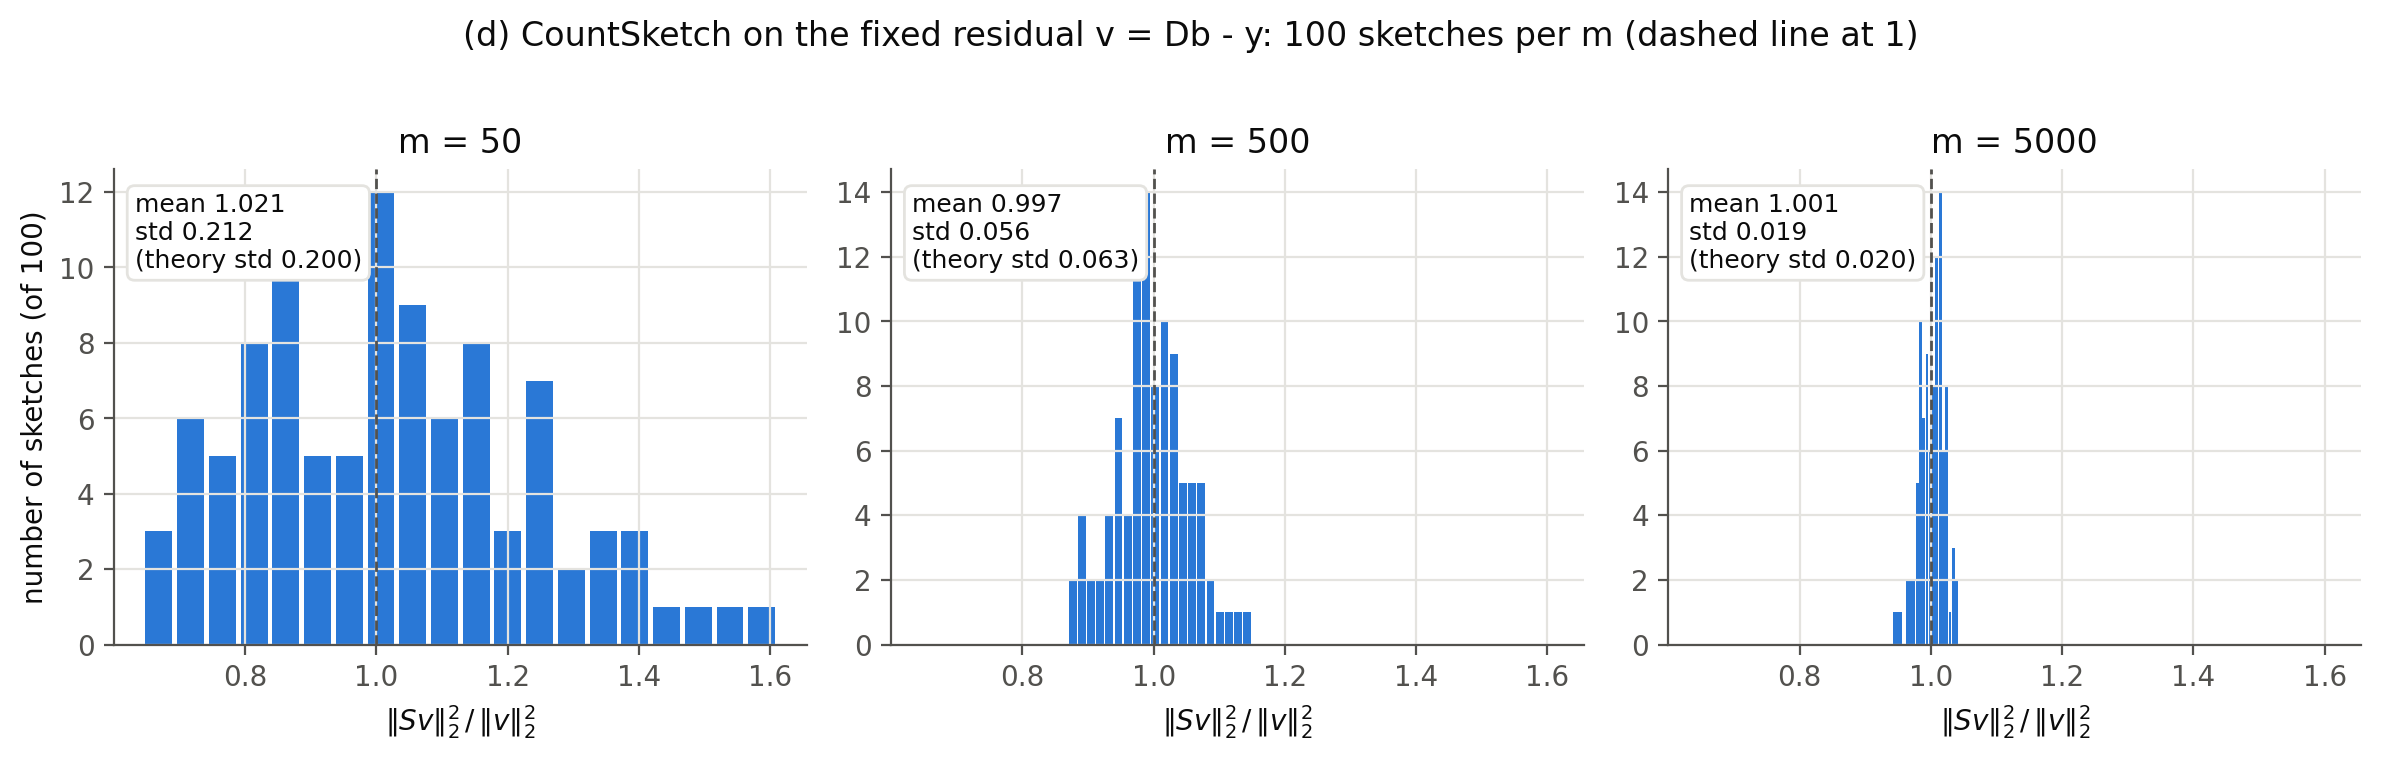
\includegraphics[width=\textwidth]{q2d_histograms.png}
\caption{Histograms of the 100 values of $\|Sv\|^2/\|v\|^2$ for each $m$. The dashed line is at 1.}
\end{figure}

\begin{table}[H]
\centering
\begin{tabular}{rrrrrr}
\toprule
$m$ & Mean & Std & Theory std & Min & Max \\
\midrule
50 & 1.0206 & 0.2117 & 0.2000 & 0.6444 & 1.6112 \\
500 & 0.9966 & 0.0562 & 0.0632 & 0.8695 & 1.1497 \\
5000 & 1.0014 & 0.0195 & 0.0200 & 0.9415 & 1.0417 \\
\bottomrule
\end{tabular}
\caption{Summary of $\|Sv\|^2/\|v\|^2$ over 100 sketches. The theory std is derived below.}
\end{table}

\textbf{Mean and variance for a fixed $v$.} Write $\delta_{ik} = \mathbf{1}[h(i)=h(k)]$. Then
\[
\|Sv\|^2 = \sum_{j=1}^m \Big(\sum_{i:\,h(i)=j} \sigma_i v_i\Big)^2
= \sum_i v_i^2 + \sum_{i\ne k} \delta_{ik}\,\sigma_i\sigma_k\,v_i v_k .
\]
Since $\mathbb{E}[\sigma_i\sigma_k] = 0$ for $i \ne k$, $\mathbb{E}\|Sv\|^2 = \|v\|^2$, so CountSketch is
unbiased. The cross terms of different pairs are uncorrelated (because of the random signs) and
$\Pr[h(i)=h(k)] = 1/m$, so
\[
\operatorname{Var}\|Sv\|^2 = 4\sum_{i<k}\frac{v_i^2v_k^2}{m} = \frac{2}{m}\big(\|v\|_2^4 - \|v\|_4^4\big),
\qquad
\operatorname{std}\frac{\|Sv\|^2}{\|v\|^2} = \sqrt{\frac{2}{m}\Big(1 - \frac{\|v\|_4^4}{\|v\|_2^4}\Big)}
\approx \sqrt{\frac{2}{m}} .
\]
Here $\|v\|_4^4/\|v\|_2^4 = 1.6\times10^{-4}$ ($v$ is spread over many rows), so the theory std is $\sqrt{2/m}$ in
practice.

\textbf{Results.} The mean is 1 up to sampling error for every $m$. The standard deviation is 0.212,
0.056 and 0.019 for $m = 50$, $500$ and $5000$, close to $\sqrt{2/m} = 0.200$, $0.063$ and $0.020$.

\textbf{How the spread changes with $m$.} The spread shrinks like $1/\sqrt{m}$: every time $m$ grows 10 times,
the histogram gets about $\sqrt{10} \approx 3.2$ times narrower. The range goes from
0.64--1.61 at $m = 50$ to 0.942--1.042 at $m = 5000$. By Chebyshev,
$\Pr\big[\,\big|\|Sv\|^2/\|v\|^2 - 1\big| > \varepsilon\big] \le 2/(m\varepsilon^2)$, so
$m = 2/(\delta\varepsilon^2)$ rows keep the length of one vector within $1 \pm \varepsilon$ with probability
$1-\delta$. This is the JL guarantee of CountSketch. Its dependence on $\delta$ is worse than the
$\log(1/\delta)$ of a Gaussian, which is the price of having only one nonzero per column.

Compare this with (b): there $S$ has to preserve a whole 113-dimensional subspace at once, not one vector.
That is why (b) needs $m$ much larger than $r$, while here $m = 50$ is already fairly accurate.

% ---------------- (e) ----------------
\subsection*{(e)}

\begin{enumerate}
    \item \textbf{Choose the subset once.} Draw 50{,}000 row indices uniformly without replacement with a
    fixed-seed generator. $D'$ is $50{,}000 \times 116$ with $\operatorname{rank}(D') = 108$, because some rare
    categories do not occur in the subset. The same subset is used for both sketches and all 5 runs.
    \item \textbf{Full solution on the subset.} $b' = \arg\min_a \|D'a-y'\|^2$ with \texttt{lstsq} gives
    Loss$(D',y',b') = 231.19$.
    \item \textbf{Sketch with $m = 500$}, with a new $S$ in each of 5 runs: (i) a CountSketch as in (b); (ii) a
    dense $S \in \mathbb{R}^{500\times 50000}$ with i.i.d.\ $N(0,1/m)$ entries
    (\texttt{rng.normal(0, 1/np.sqrt(m), size=(m, 50000))}), with $SD'$ and $Sy'$ computed by matrix products.
    We time drawing $S$ and forming $SD'$ and $Sy'$, then solve for $\tilde a$ and compute
    Loss$(D',y',\tilde a)/\text{Loss}(D',y',b')$.
\end{enumerate}

\begin{table}[H]
\centering
\begin{tabular}{lrrrr}
\toprule
 & \multicolumn{2}{c}{CountSketch} & \multicolumn{2}{c}{Gaussian} \\
\cmidrule(lr){2-3}\cmidrule(lr){4-5}
Run & Time (ms) & Ratio & Time (ms) & Ratio \\
\midrule
1 & 54.4 & 1.2456 & 244.9 & 1.2916 \\
2 & 48.8 & 1.3376 & 254.6 & 1.2585 \\
3 & 47.3 & 1.2798 & 219.3 & 1.2728 \\
4 & 48.0 & 1.2163 & 207.1 & 1.2102 \\
5 & 63.7 & 1.3719 & 257.2 & 1.2510 \\
\midrule
Mean & 52.4 & 1.2903 & 236.6 & 1.2568 \\
\bottomrule
\end{tabular}
\caption{Time to draw $S$ and form $SD'$, $Sy'$, and the ratio Loss$(D',y',\tilde a)/\text{Loss}(D',y',b')$,
on the 50{,}000-row subset with $m = 500$. The Gaussian theory gives a mean ratio of
$1 + r'/(m-r'-1) = 1.276$, where $r' = \operatorname{rank}(D') = 108$.}
\end{table}

As an extra check for the last question, we also ran each sketch once on the full $D$ with $m = 500$:

\begin{table}[H]
\centering
\small
\begin{tabular}{lccc}
\toprule
Sketch on the full $D$ & Time to draw $S$, form $SD$, $Sy$ & Storage for $S$ & Ratio \\
\midrule
CountSketch & 0.47 s & 7.9 MB ($h$ and $\sigma$) & 1.267 \\
Dense Gaussian & 3.00 s & 1{,}976 MB & 1.326 \\
\bottomrule
\end{tabular}
\caption{One run of each sketch on the full $D$, $m = 500$. Ratio $=$ Loss$(D,y,\tilde a)/L^*$.}
\end{table}

\textbf{Comparison.} On the 50{,}000-row subset the two sketches are about equally accurate (mean ratio
1.290 for CountSketch and 1.257 for the Gaussian, against 1.276 from the Gaussian theory), but
CountSketch is 4.5 times faster to draw and apply (52~ms against 237~ms). The Gaussian's
time goes into drawing $500 \cdot 50{,}000 = 2.5\times10^7$ normal numbers and the dense product
($m \cdot 50{,}000 \cdot d \approx 2.9\times10^9$ operations). CountSketch needs $10^5$ random numbers and one
pass over the $5.8\times10^6$ entries of $D'$.

\textbf{Which one we would use on the full $D$: CountSketch.}
\begin{itemize}
    \item \textbf{Time.} A dense $S$ for the full $D$ is $500 \times 494{,}021$, so applying it costs
    $m\,n\,d \approx 2.9\times10^{10}$ operations, against $nd \approx 5.7\times10^7$ for CountSketch. We measured
    0.47~s against 3.00~s (6.4 times faster). The gap is smaller than the operation count
    suggests only because dense matrix products are very fast.
    \item \textbf{Memory.} The dense $S$ alone takes 1.98 GB in float64. CountSketch only stores $h$ and
    $\sigma$ (7.9 MB).
    \item \textbf{Accuracy.} At $m = 500 \approx 4.4\,r$ both have about the same accuracy (see the two
    tables above).
    \item \textbf{One pass.} Each row only needs its own $h(i)$ and $\sigma(i)$, so $SD$ can be built while
    reading the rows one by one. For sparse data it costs $O(\operatorname{nnz}(D))$.
\end{itemize}
One caveat: the worst-case theory needs a larger $m$ for CountSketch ($O(r^2/\varepsilon^2)$) than for a
Gaussian ($O(r/\varepsilon^2)$). If a guarantee at a small $m$ were needed, one could apply a CountSketch first
and then a small Gaussian sketch to $SD$, which keeps the speed of both.

\textbf{Sources used for Question 2.}
\begin{itemize}
    \item CSE558 Lectures 18--20 (the JL lemma and JL for $k$-means).
    \item K. L. Clarkson and D. P. Woodruff, \emph{Low rank approximation and regression in input sparsity
    time}, STOC 2013. \url{https://arxiv.org/abs/1207.6365}
    \item D. P. Woodruff, \emph{Sketching as a tool for numerical linear algebra}, 2014.
    \url{https://arxiv.org/abs/1411.4357}
\end{itemize}



% ================= REFERENCES =================
\section*{Discussion and references}

Discussed with: \fillme{[names of other groups, or ``none'']}

URLs used:
\begin{itemize}
    \item \url{https://scikit-learn.org/stable/modules/generated/sklearn.cluster.KMeans.html}
    \item \url{https://scikit-learn.org/stable/modules/generated/sklearn.datasets.fetch_kddcup99.html}
    \item \fillme{[add any other URL you used]}
\end{itemize}

\end{document}
